
\begin{justify}
    \section{Introdução}
    A popularização do computador pessoal e do acesso à internet ao longo dos anos fomentou possibilidades inimagináveis. Com o advento da
    internet 2.0, surge um novo comportamento onde usuários começavam a ter uma prática social online de armazenar e disponibilizar fotos em
    redes sociais, criar blogs com facilidade sem necessidade de compreender como desenvolver um website ou como funciona um banco de dados,
    fomentando grandes empresas a enxergar nessa tendência que surgia na utilização da internet, modelos possível de plataforma e serviços que
    evoluiríam o acesso a este tipo de prática social de forma mais ampla. Isso evidenciou uma nova demanda por serviços onde o usuário passa a
    ser também consumidor.

    Esta evolução dependia não apenas da disponibilidade de novos tipos de serviço, mas também da evolução da infraestrutura de virtualização e
    comunicação de sistemas disponibilizados na internet para trazer ao mundo a possibilidade de manter grandes aplicações online, de forma
    escalável dando surgimento a modelos de serviços que contemplem uma forma mais ágil de acesso onde a informação precisa estar presente, ao
    alcance das mãos, independente da posição geográfica do meio de acesso, desde que este tenha os requisitos mínimos para que seja possível
    acessar o serviço que entrega praticidade e segurança ao cliente. 

    A partir dessa necessidade surge o conceito de Computação em Nuvem (CN), que de acordo com (CARISSIMI, 2015) “é um modelo de negócio
    onde um usuário paga apenas pelo o que consome de recursos (modelo pay-as-you-go) e o provedor do serviço mantém uma infraestrutura física
    ( data center )”, estrutura essa que além de trazer complexidade e poder de processamento de forma abstrata, traz também segurança, baixo
    custo e novos modelos de serviço que podem ser explorados tanto pelos usuários finais, bem como empresas que desejam disponibilizar um tipo
    de aplicação própria, como uma rede social, como um serviço. 
    Este nicho de “serviço como serviço” é definido de Software as a Service (SaaS), que consome de outros modelos de serviço relacionados à CN,
    como podemos observar na figura abaixo:
        
    \begin{Center}
    \begin{figure}[h]
        \centering
        \caption{Fonte}
        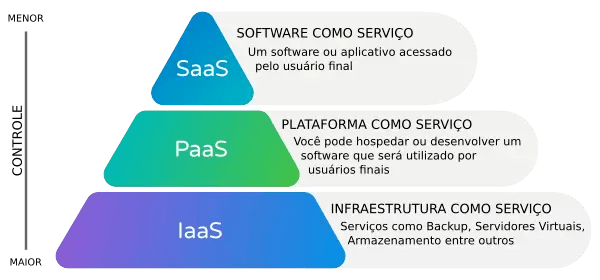
\includegraphics[scale=0.5]{iaas-paas-saas}
        \label{fig:iaas-paas-saas}
    \end{figure}
    \footnotesize{Fonte: Blog Tecnomega, 2021}
    \end{Center}

\end{justify}

\begin{justify}
    Observando a FIGURA 1, verificamos que para se disponibilizar um SaaS uma entidade depende também das estruturas de Plataforma como
    Serviço (PaaS) e principalmente da base de Infraestrutura como Serviço(IaaS), mesmo que a própria entidade seja dona de toda estrutura que o
    SaaS tenha como base, o modelo de CN se mantém o mesmo.

    Com a praticidade do acesso à estrutura CN e seus modelos de serviço deram possibilidade a surgirem também outros modelos de estrutura,
    variantes do SaaS, apenas para afirmar o tipo de serviço ofertado. Este modelo pode ser definido como “X” as a Service e é neste formato que
    grandes empresas do mundo dos games apostam para revolucionar a forma como este tipo de entretenimento pode ser mais acessível à
    diversas classes sociais, horizontalizando o acesso e aumentando a lucratividade uma vez que, o custo em se adquirir uma mídia física contendo
    um títilo de jogo, ou até mesmo no futuro, a necessidade a ter um hardware robusto e caro, fica amortizado pela própria plataforma que
    disponibilizará o possível Game as a Service (GaaS).
\end{justify}